\documentclass[10pt]{article}
\makeatletter
\usepackage[numbered,autolinebreaks,useliterate]{mcode}
\usepackage{textcomp}
\usepackage{verbatim}
\usepackage{lmodern}
\usepackage{comment}
\excludecomment{Answ}
\usepackage{listings}
\usepackage{color} %red, green, blue, yellow, cyan, magenta, black, white
\definecolor{mygreen}{RGB}{28,172,0} % color values Red, Green, Blue
\definecolor{mylilas}{RGB}{170,55,241}
\renewcommand\paragraph{\@startsection{paragraph}{4}{\z@}%
            {-2.5ex\@plus -1ex \@minus -.25ex}%
            {1.25ex \@plus .25ex}%
            {\normalfont\normalsize\bfseries}}
\makeatother
\usepackage{gensymb}
\setcounter{secnumdepth}{4}
\usepackage{amsmath}
%\usepackage{mathtools}
\usepackage{graphicx}
\usepackage{slashed}
\usepackage{lineno}
\usepackage{latexsym}
\usepackage{subfigure}
\usepackage{amssymb}
\newtheorem{thm}{Theorem}[section]
\newtheorem{cor}[thm]{Corollary}
\newtheorem{lem}[thm]{Lemma}
\usepackage[numbers,sort]{natbib}
\usepackage{enumerate}
\newcommand{\bb}{\begin{equation}}
\newcommand{\ee}{\end{equation}}
\newtheorem{defin}{Definition}
\usepackage{multirow}
\usepackage{ctable}
\usepackage{bm}
\usepackage{enumerate}
\newcommand{\D}[2]{\frac{\partial #1}{\partial #2}}
\newcommand{\DD}[2]{\frac{\partial^2 #1}{\partial #2^2}}
\newcommand{\rd}{\text{ d}}
\newcommand{\disk}{}
\usepackage{framed}
\newcommand{\see}[1]{(see Figure \ref{#1})}
\newcommand{\fig}[1]{Figure \ref{#1}}
\newcommand{\figs}[2]{figures \ref{#1} and \ref{#2}}
\newcommand{\sect}[1]{Section \ref{#1}}
\newcommand{\app}[1]{Appendix \ref{#1}}
\newcommand{\chap}[1]{Chapter \ref{#1}}
\newcommand{\eqn}[1]{equation \eqref{#1}}
\newcommand{\eqns}[2]{equations \eqref{#1} and \eqref{#2}}
\newcommand{\eqnto}[2]{equations \eqref{#1}-\eqref{#2}}
%\usepackage{authblk}
\usepackage{url}
\usepackage{hyperref}
\usepackage{soul}
\newcommand{\eg}{\emph{e.g.} }
\newcommand{\bn}{\bm{n}}
\newcommand{\bu}{\bm{u}}
\newcommand{\ie}{\emph{i.e.} }
\newcommand{\Chapter}[1]{\chapter{#1}\label{#1}}
\newcommand{\Section}[1]{\section{#1}\label{#1}}
\newcommand{\Subsection}[1]{\subsection{#1}\label{#1}}
\newcommand{\Subsubsection}[1]{\subsubsection{#1}\label{#1}}
\newcommand{\Appendix}[1]{\appendix{#1}\label{#1}}
\usepackage[margin=1.5cm,centering]{geometry}
\usepackage[geometry]{ifsym}
\makeatletter
\newcommand\restr[2]{{% we make the whole thing an ordinary symbol
  \left.\kern-\nulldelimiterspace % automatically resize the bar with \right
  #1 % the function
  \vphantom{\big|} % pretend it's a little taller at normal size
  \right|_{#2} % this is the delimiter
  }}
\def\url@leostyle{%
  \@ifundefined{selectfont}{\def\UrlFont{\sf}}{\def\UrlFont{\small\ttfamily}}}
\makeatother
\urlstyle{leo}
\usepackage{multirow}
\usepackage{blkarray}
\usepackage{soul}
\usepackage{framed}
\usepackage{color}
\usepackage{setspace}
\newcommand{\ttttp}{.24\textwidth}
\newcommand{\tttp}{.32\textwidth}
\newcommand{\ttp}{.45\textwidth}
\newcommand{\tp}{.8\textwidth}
\newcommand{\tbo}{.6\textwidth}
 \usepackage[T1]{fontenc}
\usepackage[utf8]{inputenc}
\usepackage{authblk}
 \renewcommand{\l}{\left(}
\renewcommand{\r}{\right)}
%\begin{figure}[h!!!tb]
%\centering
%\subfigure[\label{Godzilla}]{\includegraphics[height=0.35\textwidth]{./Pictures/Godzilla_final_bw.png}}
%\subfigure[\label{Jaeger}]{\includegraphics[height=0.35\textwidth]{./Pictures/Jaeger_finish_bw.png}}
%\caption{\label{Monsters} The two types of monster we are going to consider are: (a) the naturally occurring Kaijus and (b) the man-made Jaegers.}
%\end{figure}
\newcounter{Counter1}

\begin{document}

\lstset{language=Matlab,%
    %basicstyle=\color{red},
    breaklines=true,%
    morekeywords={matlab2tikz},
    keywordstyle=\color{blue},%
    morekeywords=[2]{1}, keywordstyle=[2]{\color{black}},
    identifierstyle=\color{black},%
    stringstyle=\color{mylilas},
    commentstyle=\color{mygreen},%
    showstringspaces=false,%without this there will be a symbol in the places where there is a space
    numbers=left,%
    numberstyle={\tiny \color{black}},% size of the numbers
    numbersep=9pt, % this defines how far the numbers are from the text
    emph=[1]{for,end,break},emphstyle=[1]\color{red}, %some words to emphasise
    %emph=[2]{word1,word2}, emphstyle=[2]{style},    
}


\title{Problem sheet 2}
\author{Thomas E. Woolley\\Last edited on:}
\maketitle
\section{Flattening the curve}\label{Flattening the curve}
\begin{figure}[h!!!tb]
\centering
\includegraphics[width=\tp]{../../Pictures/CDC_image.jpg}
\caption{Image taken from the website of the \href{https://www.cdc.gov/hiv/covid-19/index.html}{``Centers for Disease Control and Prevention''}. \label{CDC}}
\end{figure}
Consider the SIR equations for modelling an infectious disease and assume that the parameter values are such that we are in a pandemic scenario, \ie $\rho=rS_0/a>1$,
\begin{align}
&\dot{S}=-rSI, \quad S(0)=S_0,\\
&\dot{I}=rSI-aI,\quad I(0)=I_0,\\
&\dot{R}=aI, \quad R(0)=0.
\end{align}
Note the following questions are easier if you have a good grip on the manipulations performed on the SIR model, as seen in the notes. Thus, this would be a good time to practice deriving the following quantities. However, if you are confident that you know what you are doing\footnote{Trust me, you don't.} then you can simply write down the required answers.
\begin{enumerate}
\item Write down expressions for the maximum number of infected people, $I_{\textrm{max}}$, and total number of infected people, $I_\Sigma$, in terms of $a, r, S_0, I_0$ and $S_\infty$.

\item Write down the expression that $S_\infty$ must satisfy, call this the consistency equation.

\item Plot the left- and right-hand sides of the consistency equation on the same axes with $S_\infty$ on the $x$-axis. Demonstrate that there are, generally, two possible roots and highlight which root we are interested in.\label{Graphical_question}
\setcounter{Counter1}{\value{enumi}}
\end{enumerate}

In the early stages of the corona pandemic much was made of the ``Flatten the Curve'' idea. Namely, if you can reduce the infection rate then it was reported that although it would make the disease last longer it would reduce the maximum number of infections, thus, allowing the health care system to cope  \see{CDC}.
\begin{enumerate}
\setcounter{enumi}{\value{Counter1}}
\item Consider two infection rates $r_1$, $r_2$, such that $r_1>r_2$. Show that $I_{\textrm{max}}(r_1)>I_{\textrm{max}}(r_2)$.

Hint 1: we are considering a pandemic situation, so the reproduction number, $\rho$, is greater than one.

Hint 2: consider the derivative of $I_{\textrm{max}}(r)$ with respect to $r$.
\setcounter{Counter1}{\value{enumi}}
\end{enumerate}
As shown in the last question reducing the infection rate does reduce the maximum number of infections. However, it also extends the infection period \see{CDC}. Thus, are we sure that the total number of infectives is smaller? For example, instead of infecting 10 people in week 1 are we infecting 1 person per week and making the infection last 10 weeks?  Namely, are we just delaying the inevitable, or does reducing the infection rate actually reduce total number of infectives?
\begin{enumerate}
\setcounter{enumi}{\value{Counter1}}
\item  Show that if $r_1>r_2$ then $I_{\Sigma}(r_1)>I_{\Sigma}(r_2)$.


Hint 1: Approach this equation graphically using the result from question \ref{Graphical_question}.
\end{enumerate}

\begin{Answ}
\subsection{Answers}
\begin{enumerate}
\item Since we are considering the pandemic scenario then from the lecture notes
\bb
I_{\textrm{max}}=I_0+S_0-\frac{a}{r}+\frac{a}{r}\ln\l\frac{a}{rS_0}\r,\label{Imax}
\ee
\bb
I_{\Sigma}=R_\infty=S_0+I_0-S_\infty=N-S_\infty,
\ee
where all terms are defined as in the notes.

\item 
\bb
S_\infty-\frac{a}{r}\ln\l S_\infty\r=N-\frac{a}{r}\ln\l S_0\r.\label{Consistency}
\ee
\item See \fig{Consistency_equation}. The two roots are circled in red and labelled $S_{L\infty}<S_{R\infty}$. Since the susceptible population is always decreasing $S_{L\infty}$ is the correct root to choose.
\begin{figure}[h!!!tb]
\centering
\includegraphics[width=\ttp]{../../Pictures/Consistency_equation}
\caption{\label{Consistency_equation} Plotting the left- and right-hand sides of \eqn{Consistency}.}
\end{figure}

\item Take the derivative of \eqn{Imax} with respect to $r$,
\bb
\frac{\rd I_{\textrm{max}}}{\rd r}=\frac{a}{r^2}-\frac{a}{r^2}\ln\l\frac{a}{rS_0}\r-\frac{a}{r^2}=-\frac{a}{r^2}\ln\l\frac{a}{rS_0}\r.
\ee
Since we are in a pandemic $\rho=rS_0/a>1$, meaning that $0<a/rS_0<1$, thus $\ln\l a/rS_0\r<0$. Hence, $\rd I_{\textrm{max}}/\rd r>0$. This means $I_{\textrm{max}}$ is an increasing function with respect to $r$, which implies that if $r_1>r_2$ then $I_{\textrm{max}}(r_1)>I_{\textrm{max}}(r_2)$. Thus, proving the desired result.

\item We want to plot the left- and right-hand sides of \eqn{Consistency} for two different values of $r$. First thing to note is that all the $S_\infty-\l a/r\r\ln(S_\infty)$ curves meet at $S_\infty=1$. Further, if $r_1>r_2$ then $N-(a/r_1)\ln(S_0)>N-(a/r_2)\ln(S_0)$ and 
\bb
S_\infty-\l a/r_1\r\ln(S_\infty)>S_\infty-\l a/r_2\r\ln(S_\infty) \textrm{ for } S_\infty>1,
\ee
\bb
S_\infty-\l a/r_1\r\ln(S_\infty)<S_\infty-\l a/r_2\r\ln(S_\infty) \textrm{ for }S_\infty<1.
\ee
\fig{Flatten} illustrates all of this information on one set of axes, where we have zoomed in on the left-hand roots. Clearly we see that $S_\infty(r_1)<S_\infty(r_2)$ leading to the result that
\bb
I_{\Sigma}(r_1)=N-S_\infty(r_1)>N-S_\infty(r_2)=I_{\Sigma}(r_2).
\ee
Thus, decreasing $r$ does indeed reduce the maximum number of infectives as well as reduce the entire total number of infected. Flattening the curve is a good idea.
\begin{figure}[h!!!tb]
\centering
\includegraphics[width=\tp]{../../Pictures/Flatten_the_curve.png}
\caption{\label{Flatten} Plotting the left- and right-hand sides of \eqn{Consistency} for two different values of $r$.}
\end{figure}
\end{enumerate}
\end{Answ}

\section{Discrete dynamics}
Consider the following discrete evolution equation of a population $N_t$ at generation $t$,
\bb
N_{t+1}=\frac{bN_t^2}{1+N_t^2}-EN_t=f(N_t),\label{Nt}
\ee
where $b>2$ and $E>0$ are constants.
\begin{enumerate}
\item Suggest a biological interpretation of \eqn{Nt}.
\item Determine the three steady states of \eqn{Nt}. Define them to be $N_0<N_-\leq N_+$. You should be able to show that $N_\pm$ only exist if $E<(b-2)/2=E_M$.
\item Draw $(x,y)$ graphs of
\bb
y=\frac{bx^2}{1+x^2} \text{ and }y=Ex\label{Components}
\ee
for a variety of $b$ and $E$. Using these graphs draw three $(N_t,N_{t+1})$ plots for the three cases
\begin{enumerate}
\item $E<E_M$,
\item $E=E_M$,
\item $E>E_M$.
\end{enumerate}
\item Focusing now on the case of $E<E_M=(b-2)/2$. Show by cob-webbing, or otherwise, that the model is realistic only if the population, $N_t$, always lies between the two positive values $[N_-,N_2]$, where you should analytically derive the form of $N_2$.
\item By cobwebbing, or otherwise, discuss the stability of the steady states $N_0, N_\pm$.
\end{enumerate}




\begin{Answ}
\subsection{Answers}
\begin{enumerate}
\item The
\bb
\frac{bN^2}{1+N_t^2}
\ee
term is positive but it saturates for large $N_t$. Hence, it represents reproduction with competition. The $-EN_t$ term  suggests that a constant proportion of the population is removed during each generation. Thus, the dynamics could be harvesting of a farmed species, for example, fish stocks.
\item Steady states are when $N_t=N$ for all $t$. Thus, the steady states satisfy
\bb
N=\frac{bN^2}{1+N^2}-EN.\nonumber
\ee
By inspection $N=0$ is a solution. Call this solution $N_0$. Cancel the $N$s on both sides to get
\bb
1+E=\frac{bN}{1+N^2},\nonumber
\ee
\bb
\implies N^2(1+E)-bN+(1+E)=0,\nonumber
\ee
\bb
\implies N_\pm=\frac{b\pm\sqrt{b^2-4(1+E)^2}}{2(1+E)}.\nonumber
\ee
The roots $N_\pm$ only exist when they are real, thus,
\bb
b^2>4(1+E)^2,\nonumber
\ee
\bb
\implies b>2(1+E),\nonumber
\ee
\bb
\implies E_M=\frac{b-2}{2}>E.
\ee
\item After some sketching you should come to realise that you do not need to vary both parameters. Thus, we can cover all possible outcomes by varying $E$ \see{Discrete_dynamics}.

The top image of \fig{Discrete_dynamics} shows that as $E$ increases the line $Ex$ gets steeper. For $E<E_M$ the two curves cross three times (black and red curves in top figure). At $E=E_M$ the two curves cross twice times (black and blue curves in top figure). For $E>E_M$ the two curves cross once (black and green curves in top figure). The coloured lines in the top graph then corresponds to the coloured curves in the bottom graphs. Namely, if $E<E_M$ then $N_0, N_-$ and $N_+$ all exist. If $E=E_M$ then $N_0$ and $N_-=N_+$ exist. If $E>E_M$ then only $N_0$ exists.
\begin{figure}[h!!!tb]
\centering
\includegraphics[width=\tp]{../../Pictures/Discrete_dynamics.png}
\caption{\label{Discrete_dynamics} Plotting the two curves from \eqn{Components} and interpreting the two components into $(N_t,N_{t+1})$ graphs for various values of $E$. }
\end{figure}



\item From cobwebbing in multiple places we see that the starting points must be between $N_-$ and $N_2$ (green region in \fig{Cobwebbing}). If you start with initial conditions outside of this region (red region in \fig{Cobwebbing}) the trajectories end up going negative, which is unrealistic for a population model.
\begin{figure}[h!!!tb]
\centering
\includegraphics[width=\tp]{../../Pictures/Cobwebbing.png}
\caption{\label{Cobwebbing} Cobwebbing \eqn{Nt} in the case $E<E_M$. The green area and green cobwebs are the realistic region. The red region and red cobwebs go negative and are, thus, unrealistic. }
\end{figure}

To calculate $N_2$ we realise that it satisfies $f(N_2)=N_-$. Further, from considering \fig{Cobwebbing} we know there must be three roots $N_1<0<N_-<N_2$. We also note that, by definition, $N_-$ satisfies
\bb
N_-=\frac{bN_-^2}{1+N_-^2}-EN_-.
\ee
Using this information we derive
\bb
\frac{bN_-^2}{1+N_-^2}-EN_-=N_-=f(N)=\frac{bN^2}{1+N^2}-EN\label{N-f}.
\ee
Since we know that $N_-$ is a root we manipulate \eqn{N-f} to extract it,
\bb
\implies 0=\frac{bN_-^2}{1+N_-^2}-\frac{bN^2}{1+N^2}-E(N_-+N),\nonumber
\ee
\bb
\implies0=\frac{b}{\l 1+N_-^2\r\l 1+N^2\r}\l N_-^2\l 1+N^2\r-N^2\l 1+N_-^2\r\r-E(N_--N),\nonumber
\ee
\bb
\implies0=\frac{b}{\l 1+N_-^2\r\l 1+N^2\r}\l N_-^2-N^2\r-E(N_--N),\nonumber
\ee
\bb
\implies0=\frac{b(N_--N)(N_-+N)}{\l 1+N_-^2\r\l 1+N^2\r}-E(N_--N),\nonumber
\ee
\bb
\implies0=(N_--N)\l\frac{b(N_-+N)}{\l 1+N_-^2\r\l 1+N^2\r}-E\r.\label{Nroot}
\ee
Equation \eqref{Nroot} confirms that $N_-$ is one of the roots. Acknowledging this we can divide through by $(N_--N)$ and solve the remaining quadratic for the remaining two roots.
\bb
0=\frac{b(N_-+N)}{\l 1+N_-^2\r\l 1+N^2\r}-E,\nonumber
\ee
\begin{align}
\implies 0=&b(N_-+N)-E\l 1+N_-^2\r\l 1+N^2\r,\nonumber\\
=&E\l 1+N_-^2\r N^2-bN+E\l 1+N_-^2\r-bN_-,\nonumber\\
\implies N_{1,2}=&\frac{b\pm\sqrt{b^2-4E(1+N_-^2)\l E\l 1+N_-^2\r-bN_-\r}}{2E(1+N_-^2)}.\nonumber
\end{align}
Note we do require
\bb
b^2-4E(1+N_-^2)\l E\l 1+N_-^2\r-bN_-\r>0\label{ineq}
\ee
for $N_{1,2}$ to exist. However, from \fig{Cobwebbing} we can deduce that whenever $N_-$ exists then so will $N_{1,2}$, thus satisfying $E_M>E$ will also satisfy inequality \eqref{ineq}.


\end{enumerate}
\end{Answ}
\section{Cobwebbing in Matlab}
The code below simulates the dynamics as presented in question 2. Once again, you can download this code from learning central, or copy and paste it from here.


Simulating discrete dynamics is, in some ways, easier than simulating ODEs. Given a value for $N_t$ and a function $f$ you simply evaluate $f(N_t)$ to calculate $N_{t+1}$. Thus, most of the cobwebbing code below is for plotting purposes. The actual calculation step occurs in lines 43-46.

Have a go at altering the parameters $b$ and $E$ in lines 9-10. Equally, change the initial conditions in lines 36-38 to see where you will end up.

If you are really feeling adventurous, alter the code to work with the discrete logistic equation and simulate chaos!
\lstset{numbers=none}
\begin{lstlisting}
%% Ensure we start from a blank slate
clear all
close all
clc

%% Initialise variables
fs=15; % Set fontsize

b=4;
E=0.8;

Np=(b+sqrt(b^2-4*(1+E)^2))/(2*(1+E)); %N+ from question 2.
Nn=(b-sqrt(b^2-4*(1+E)^2))/(2*(1+E)); %N- from question 2.
N1=(b-sqrt(b^2-4*E*(1+Nn^2)*(E*(1+Nn^2)-b*Nn)))/(2*E*(1+Nn^2)); %N1 from question 2.
N2=(b+sqrt(b^2-4*E*(1+Nn^2)*(E*(1+Nn^2)-b*Nn)))/(2*E*(1+Nn^2)); %N2 from question 2.

%% Set up the basic plotting space
N=linspace(-1,8);

hold on
plot(N,N,'k') % Plot N(t)=N(t+1)
plot(N,b*N.^2./(1+N.^2)-E*N,'b') % Plot N(t+1)=f(N(t))
plot(N,Nn*ones(1,length(N)),'--k','linewidth',1) % Plot N(t+1)=N-
plot([N1 N1],[0 Nn],'--k','linewidth',1) % Plot N(t)=N1
plot([Nn Nn],[0 Nn],'--k','linewidth',1) % Plot N(t)=N-
plot([N2 N2],[0 Nn],'--k','linewidth',1) % Plot N(t)=N2
axis([0 5 0 2])
xlabel('$N_t$')
ylabel('$N_{t+1}$')

%% Calculate the cobweb diagram
% The Cobweb(x1,x2,x3,x4) function has 4 arguments x1-x4.
% x1 is the initial point from which the cobweb starts.
% x2 and x3 are the parameters b and E, respectively.
% x4 is the colour of the cobweb.
Cobweb(3,b,E,'b')
Cobweb(0.5,b,E,'r')
Cobweb(4.5,b,E,'r')
set(gca,'fontsize',fs) % Set fontsize.

function Cobweb(N0,b,E,c)
% The following for loop computes the first 100 iteration values.
Nt(1)=N0;
for i=1:100
    Nt(i+1)=b*Nt(i)^2/(1+Nt(i)^2)-E*Nt(i);
end


% The following code plots the cobweb.
plot([Nt(1) Nt(1)],[0 Nt(2)],c,'linewidth',1)
for i=1:100-2
    plot([Nt(i) Nt(i+1)],[Nt(i+1) Nt(i+1)],c,'linewidth',1)
    plot([Nt(i+1) Nt(i+1)],[Nt(i+1) Nt(i+2)],c,'linewidth',1)
end
end
\end{lstlisting}

\section*{Exam Revision}
\section{A different infection model}
An animal population is prone to a fatal disease. There is a limited vaccine that creates immunity in the susceptible population but has no effect on infected animals. The higher the number of infected animals observed, the more vigorously vaccinations are administered.

Let $I$ denote the number of infected animals, $S$ the number of susceptible animals, $V$ the number of vaccinated animals and $R$ the number of dead animals. An ordinary differential equation description of these interactions can be written
\begin{align}
\frac{\rd S}{\rd T} =&-\beta SI-pSI,\\
\frac{\rd I}{\rd T} =&\beta SI-aI,\\
\frac{\rd R}{\rd T} =&aI,\\
\frac{\rd V}{\rd T} =&pSI.
\end{align}

\begin{enumerate}

\item Explain the biological interpretation of each of the terms in the model.

\item Non-dimensionalise the model to give
\begin{align}
\frac{\rd s}{\rd t} =&-si(1+\eta),\label{Nondims1}\\
\frac{\rd i}{\rd t} =&i(s-1),\\
\frac{\rd r}{\rd t} =&i,\\
\frac{\rd v}{\rd t} =&\eta si.\label{Nondimv1}
\end{align}
where $s, i, r, v$ and $t$ are the non-dimensional variables corresponding  to the upper-case dimensional variables. The parameter $\eta>0$ should be given in terms of $a, \beta$ and $p$.
\setcounter{Counter1}{\value{enumi}}
\end{enumerate}

Suppose that the initial conditions are
\bb
s(0)=s_0, i(0)=i_0, r(0)=0, v(0)=0,\nonumber
\ee
where $s_0, i_0>0$ and assume that $i\rightarrow 0$ as $t\rightarrow\infty$.


\begin{enumerate}
\setcounter{enumi}{\value{Counter1}}
\item Show 
\bb
s+i+r+v=\textrm{constant},\label{Conserved}
\ee
where the constant should be defined.
\item What does \eqn{Conserved} mean? Is this physically correct?
\item Define $r_\infty=\lim_{t\rightarrow\infty}r(t)$ and $s_\infty=\lim_{t\rightarrow\infty}s(t)$. What do $r_\infty$ and $s_\infty$ represent?
\item By considering $\rd i/\rd s$ and $\rd v/\rd s$ show that
\bb
r_\infty=\frac{1}{1+\eta}\ln\l\frac{s_0}{s_\infty}\r.
\ee
\end{enumerate}

\begin{Answ}
\subsection{Answers}
\begin{enumerate}
\item Susceptibles become infected at a rate proportional to their interaction rate with infectives with rate constant $\beta$. Susceptibles are vaccinated at a rate proportional to their interaction rate with infectives with rate constant $p$. Infectives die at a rate proportional to their population size, with rate constant $a$.



\item For each variable sub in the form $P=[P]p$, where $P$ is the dimensional variable, $p$ is the non-dimensional variable and $[P]$ is the dimensional scale.
\begin{align}
\frac{[S]}{[T]}\frac{\rd s}{\rd t} =&-\beta [S][I]si\l 1+\frac{p}{\beta}\r,\label{Nondims}\\
\frac{[I]}{[T]}\frac{\rd i}{\rd t} =&[I][S]i\beta\l s-\frac{a}{\beta[S]}\r,\\
\frac{[R]}{[T]}\frac{\rd r}{\rd t} =&a[I]i,\\
\frac{[V]}{[T]}\frac{\rd v}{\rd t} =&p[S][I]si.\label{Nondimv}
\end{align}
Comparing \eqnto{Nondims}{Nondimv} with \eqnto{Nondims1}{Nondimv1} we see that
\bb
\frac{1}{[T]}=\beta[I],\quad \eta=\frac{p}{\beta},\quad \frac{1}{[T]}=\beta[S],\quad \frac{a}{\beta[S]}=1,\quad\frac{[R]}{[T]}=a[I],\quad \frac{p[S][I][T]}{[V]}=\eta.
\ee
So,
\bb
[S]=\frac{a}{\beta}=[I]=[R]=[V], \quad [T]=\frac{1}{a},\quad \eta=\frac{p}{\beta}.
\ee
\item Adding \eqnto{Nondims}{Nondimv} together the right-hand side disappears. Integrating with respect to time gives \eqn{Conserved}. Since the constant holds for all time it is true initially, thus
\bb
s(t)+i(t)+r(t)+v(t)=s_0+i_0
\ee
for all $t\geq 0$.

\item The entire population is conserved, thus, an individual can only transition between one of four states: susceptible, infected, removed (dead), vaccinated. Note this means that there is no birth, nor death from other causes. Of course this is not physically correct, but we are assuming that the disease occurs over a short enough time scale that births and deaths via other sources do not influence the result greatly.

\item $r_\infty$ is the (non-dimensionalised) population that has died from the virus. $s_\infty$ is the (non-dimensionalised) population that is susceptible after the infection has disappeared.

\item Using \eqn{Conserved} we know that
\bb
s_\infty+r_\infty+v_\infty=s_0+i_0.\label{inftyconstant}
\ee
Further
\bb
\frac{\rd i}{\rd s}=-\frac{i(s-1)}{si(1+\eta)} \text{ and }\frac{\rd v}{\rd s}=-\frac{\eta is}{si(1+\eta)}.\nonumber
\ee
So,
\bb
\int^0_{i_0}1+\eta\rd i=\int^{s_\infty}_{s_0}\frac{1}{s}-1\rd s \text{ and } \int^{v_\infty}_0 \rd v=\int^{s_\infty}_{s_0}-\frac{\eta}{1+\eta}\rd s,\nonumber
\ee
resulting in
\bb
-(1+\eta)i_0=\ln\l\frac{s_\infty}{s_0}\r-(s_\infty-s_0)\text{ and }v_\infty=\frac{\eta}{1+\eta}\l s_0-s_\infty\r.\label{i0vinfty}
\ee
Substituting $i_0$ and $v_\infty$ from equations \eqref{i0vinfty} into \eqn{inftyconstant} then gives
\begin{align}
r_\infty=&s_0-s_\infty-\frac{s_0-s_\infty}{1+\eta}-\frac{1}{1+\eta}\ln\l\frac{s_\infty}{s_0}\r-\frac{\eta}{1+\eta}(s_0-s_\infty),\nonumber\\
=&(s_0-s_\infty)\l 1- \frac{1}{1+\eta}-\frac{\eta}{1+\eta}\r-\frac{1}{1+\eta}\ln\l\frac{s_\infty}{s_0}\r,\nonumber\\
=&\frac{1}{1+\eta}\ln\l\frac{s_0}{s_\infty}\r.
\end{align}
\end{enumerate}
\end{Answ}







\section{Discrete Ricker model}
Suppose that the evolution of a population can be described by a discrete-time Ricker
model of the form
\bb
N_{t+1} = N_t \exp\l r\l 1-\frac{N_t}{K}\r\r=f(N_t),
\ee
where $r,K>0$ are constants.
\begin{enumerate}
\item Describe the biological interpretation of the model.
\item Determine any non-negative steady states and their linear stability.
\setcounter{Counter1}{\value{enumi}}
\end{enumerate}

\noindent Let us now fix $K=1$.

\begin{enumerate}
\setcounter{enumi}{\value{Counter1}}
\item Construct a cobweb map for the model when $0<r<2$ and discuss the global qualitative behaviour of the solutions.


\item Using \fig{Ricker}, or otherwise, specify the steady states and their stability in the three cases of the discrete Ricker model when $r=1$, 2.1 and 3.
\begin{figure}[h!!!tb]
\centering
\subfigure[$r=1$\label{r_1}]{\includegraphics[width=\tp]{../../Pictures/Ricker_r1.png}}
\subfigure[$r=2.1$\label{r_21}]{\includegraphics[width=\tp]{../../Pictures/Ricker_r21.png}}
\subfigure[$r=3$\label{r_3}]{\includegraphics[width=\tp]{../../Pictures/Ricker_r3.png}}
\caption{\label{Ricker}Plot of the discrete Ricker model for different values of $r$ (specified beneath each figure). In all case $K=1$.}
\end{figure}
\end{enumerate}

\begin{Answ}
\subsection{Answers}
\begin{enumerate}
\item It is a reproduction model with rate $r$ and carrying capacity $K$.
\item Solving
\bb
N=N\exp\l r\l 1-\frac{N}{K}\r\r,
\ee
gives $N=0,K$.
The stability of the steady states are derived from considering the size of $f'(N)$ at the steady states,
\begin{align}
f'(N)&=\frac{\rd}{\rd N}\l N\exp\l r\l 1-\frac{N}{K}\r\r\r,\\
&=\exp\l r\l 1-\frac{N}{K}\r\r \l 1-\frac{Nr}{K}\r.
\end{align}
Thus, $f'(0)=\exp(r)>1$ for all $r>0$, hence 0 is always unstable. Further,
\bb
f'(K)=1-r.
\ee
Thus, $N=K$ is stable for $0<r<2$ and unstable for $r>2$.
\item See the answer to $r=1$ below. Note the point of this question was that you should try and sketch the curve yourself, before copying the printed versions.


\item Firstly, we note that the steady is independent of $r$, so, when $K=1$, the steady states are always $N=0$ and 1.
\begin{itemize}
\item When $r<2$ the analysis and the cobweb both suggest that $N=0$ is unstable and $N=1$ is globally stable.

\item When $r>2$ the analysis suggest that $N=1$ is unstable but we do not know what happens then. From the cobweb we see that when $r=2.1$ the trajectories tend to a period 2 oscillatory state.

\item When $r=3$ the cobweb suggests a chaotic trajectory.


\end{itemize}

\begin{figure}[h!!!tb]
\centering
\subfigure[$r=1$\label{r_1_cobweb}]{\includegraphics[width=\ttp]{../../Pictures/Ricker_cobweb_r1.png}}
\subfigure[$r=2.1$\label{r_21_cobweb}]{\includegraphics[width=\ttp]{../../Pictures/Ricker_cobweb_r21.png}}
\subfigure[$r=3$\label{r_3_cobweb}]{\includegraphics[width=\ttp]{../../Pictures/Ricker_cobweb_r3.png}}
\caption{\label{Ricker_cobweb} Cobwebbed solutions of the discrete Ricker model for different values of $r$ (specified beneath each figure). In all case $K=1$. The red, green and magenta lines show trajectories with different starting points. Red starts at $N_0=0.1$, green starts at $N_0=3$ and magenta starts at $N_0=4$.}
\end{figure}
\end{enumerate}
\end{Answ}
\end{document}


\begin{figure}[h!!!tb]
\centering
\subfigure[$r=1$\label{r_1_cobweb}]{\includegraphics[width=\ttp]{../../Pictures/Ricker_cobweb_r1.png}}
\subfigure[$r=2.1$\label{r_21_cobweb}]{\includegraphics[width=\ttp]{../../Pictures/Ricker_cobweb_r21.png}}
\subfigure[$r=3$\label{r_3_cobweb}]{\includegraphics[width=\ttp]{../../Pictures/Ricker_cobweb_r3.png}}
\caption{\label{Ricker_cobweb} Cobwebbed solutions of the discrete Ricker model for different values of $r$ (specified beneath each figure). In all case $K=1$. The red, green and magenta lines show trajectories with different starting points. Red starts at $N_0=0.1$, green starts at $N_0=3$ and magenta starts at $N_0=4$.}
\end{figure}
\end{enumerate}

